\documentclass{article}

\usepackage{tikz}
\usetikzlibrary{automata, positioning}
\begin{document}
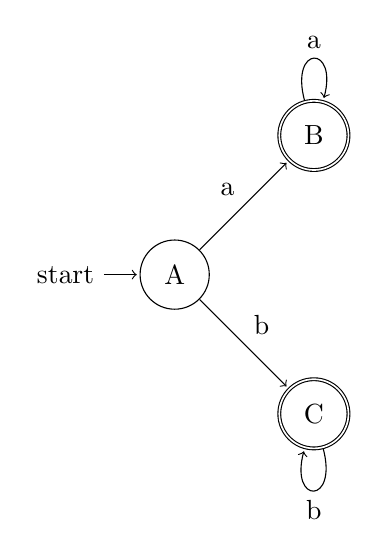
\begin{tikzpicture}[shorten >= 1pt, node distance = 2.5cm, on grid, auto]
  \node[state, initial] (A) {A};
  \node[state, accepting] (B) [above right=of A] {B};
  \node[state, accepting] (C) [below right=of A] {C};
  \path[->]
    (A) edge node {a} (B)
        edge node {b} (C)
    (B) edge [loop above] node {a} (B)
    (C) edge [loop below] node {b} (C);
\end{tikzpicture}
\end{document}
